\documentclass{beamer}

\usepackage{graphicx}
\usepackage{color}
\usepackage{listings}

\usetheme{Boadilla}

\AtBeginSection[]{
    \begin{frame}
    \vfill
    \centering
      \usebeamerfont{title}\insertsectionhead\par%
    \vfill
    \end{frame}
}

\definecolor{darkgreen}{rgb}{0,0.6,0}
\definecolor{darkorange}{rgb}{1,0.4,0}

\lstdefinestyle{codestyle}{
    backgroundcolor=\color{white},
    commentstyle=\color{darkgreen},
    keywordstyle=\color{blue},
    numberstyle=\color{black},
    stringstyle=\color{darkorange},
    basicstyle=\ttfamily\footnotesize,
    breakatwhitespace=false,
    breaklines=true,
    captionpos=b,
    keepspaces=true,
    numbers=none,
    showspaces=false,
    showstringspaces=false,
    showtabs=false,
    breaklines=true,
}

\lstset{style=codestyle}

\title{Esplorare L'API Grafica Vulkan}
\author{Emanuele Franchi}
\date{}

\begin{document}

\begin{frame}

\titlepage

\end{frame}


% \begin{frame}
\frametitle{Vulkan Come API Grafica}
\begin{columns}

\column{.6\textwidth}

\begin{itemize}
\item Vulkan è un'API grafica cross platform di nuova generazione
\item Un'API grafica è un'interfaccia che ci permette di interagire con la GPU
\end{itemize}

\column{.2\textwidth}

\begin{figure}[ht]
    \centering
    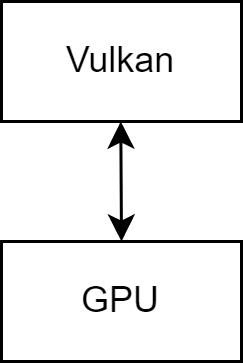
\includegraphics[scale=0.2]{images/SlidesVulkan/VulkanAPI.png}
\end{figure}

\end{columns}
\end{frame}

% \begin{frame}
\frametitle{Vulkan (2)}

\begin{itemize}
\item Successore di OpenGL
\item Anno di rilascio: 2016
\item Sviluppata usando come modello l'architettura delle GPU odierne
\item Driver molto più semplici e leggeri
\item A più basso livello rispetto ad OpenGL
\item Richiede più conoscenze da parte del programmatore
\item Più verbosa rispetto ad OpenGL
\item Può risultare in performance migliori, se il programmatore la usa coscientemente
\item Sviluppata per essere usata in un contesto multithreaded
\item Essendo così nuova, le GPU meno recenti non la supportano
\end{itemize}

\end{frame}

%
% \begin{frame}
\frametitle{Vulkan Instance}
\begin{columns}

\column{.6\textwidth}

\begin{itemize}
\item Dobbiamo creare un'istanza di Vulkan per accedere al resto dell'API
\item Quando creiamo un'istanza indichiamo i layer che vogliamo abilitare
\item I layer sono componenti opzionali
\item I layer modificano il comportamento delle funzioni dell'API
\item Per esempio, possiamo usare un layer per controllare se il nostro utilizzo dell'API non violi la specifica
\item Quando creiamo un'istanza indichiamo le estensioni d'istanza che vogliamo abilitare
\item Le estensioni aggiungono nuove funzioni all'API
\end{itemize}

\column{.4\textwidth}

\begin{figure}[ht]
    \centering
    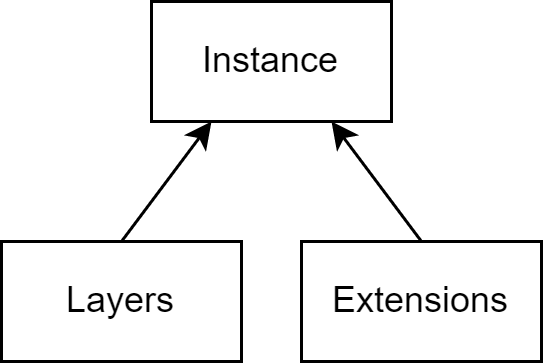
\includegraphics[scale=0.2]{images/SlidesInitializingVulkan/Instance.png}
\end{figure}

\end{columns}
\end{frame}

% \begin{frame}
\frametitle{Finestra e Vulkan Presentation Surface}
\begin{columns}

\column{.6\textwidth}

\begin{itemize}
\item Creiamo una finestra usando l'API del sistema operativo
\item Creiamo una Vulkan presentation surface per interagire con la finestra creata
\end{itemize}

\column{.2\textwidth}

\begin{figure}[ht]
    \centering
    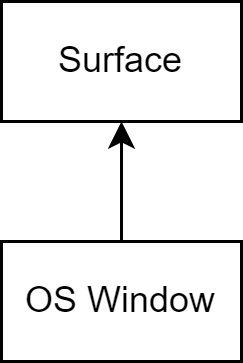
\includegraphics[scale=0.2]{images/SlidesInitializingVulkan/WindowAndSurface.png}
\end{figure}

\end{columns}
\end{frame}

% \begin{frame}
\frametitle{Selezionare Un Device Fisico}

\begin{itemize}
\item Dobbiamo selezionare la GPU che andremo a utilizzare
\item Deve supportare operazioni grafiche, quindi deve avere almeno una coda che possa eseguire tali comandi
\item Deve supportare operazioni di presentazione di immagini, quindi deve avere almeno una coda che possa eseguire tali comandi
\item Deve supportare la creazione di una swapchain
\item Deve supportare almeno una modalità di presentazione compatibile con la presentation surface che abbiamo creato precedentemente
\end{itemize}

\end{frame}

% \begin{frame}
\frametitle{Creare Un Device Logico}
\begin{columns}

\column{.6\textwidth}

\begin{itemize}
\item Per interagire con il device fisico selezionato, dobbiamo creare un device logico
\item Quando creiamo il device logico, indichiamo la creazione di una coda per eseguire comandi grafici, e una coda per eseguire comandi di presentazione
\item Una volta creato il device logico, possiamo ottenere le code richieste
\item Se una coda supporta sia operazioni grafiche che di presentazione, possiamo usarla singolarmente
\end{itemize}

\column{.2\textwidth}

\begin{figure}[ht]
    \centering
    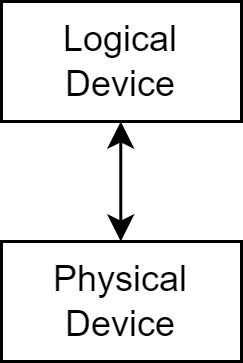
\includegraphics[scale=0.2]{images/SlidesInitializingVulkan/LogicalDevice.png}
\end{figure}

\end{columns}
\end{frame}

% \begin{frame}
\frametitle{Creare Una Swapchain}
\begin{columns}

\column{.6\textwidth}

\begin{itemize}
\item Una volta creato un device logico, lo possiamo utilizzare per creare una swapchain
\item Dobbiamo creare una swapchain per presentare immagini sulla presentation surface
\item Una swapchain crea e gestisce le immagini che saranno presentate
\item Tramite la swapchain dobbiamo specificare la modalità di presentazione che verrà usata dal presentation engine del sistema operativo
\end{itemize}

\column{.2\textwidth}

\begin{figure}[ht]
    \centering
    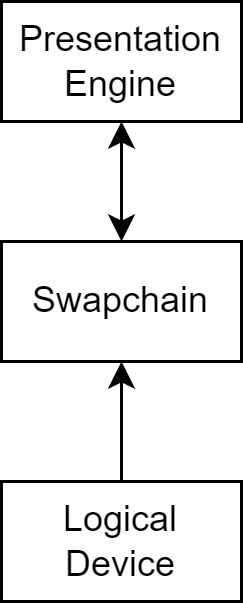
\includegraphics[scale=0.2]{images/SlidesInitializingVulkan/Swapchain.png}
\end{figure}

\end{columns}
\end{frame}

%
% \begin{frame}
\frametitle{Risultato}

\begin{figure}[ht]
    \centering
    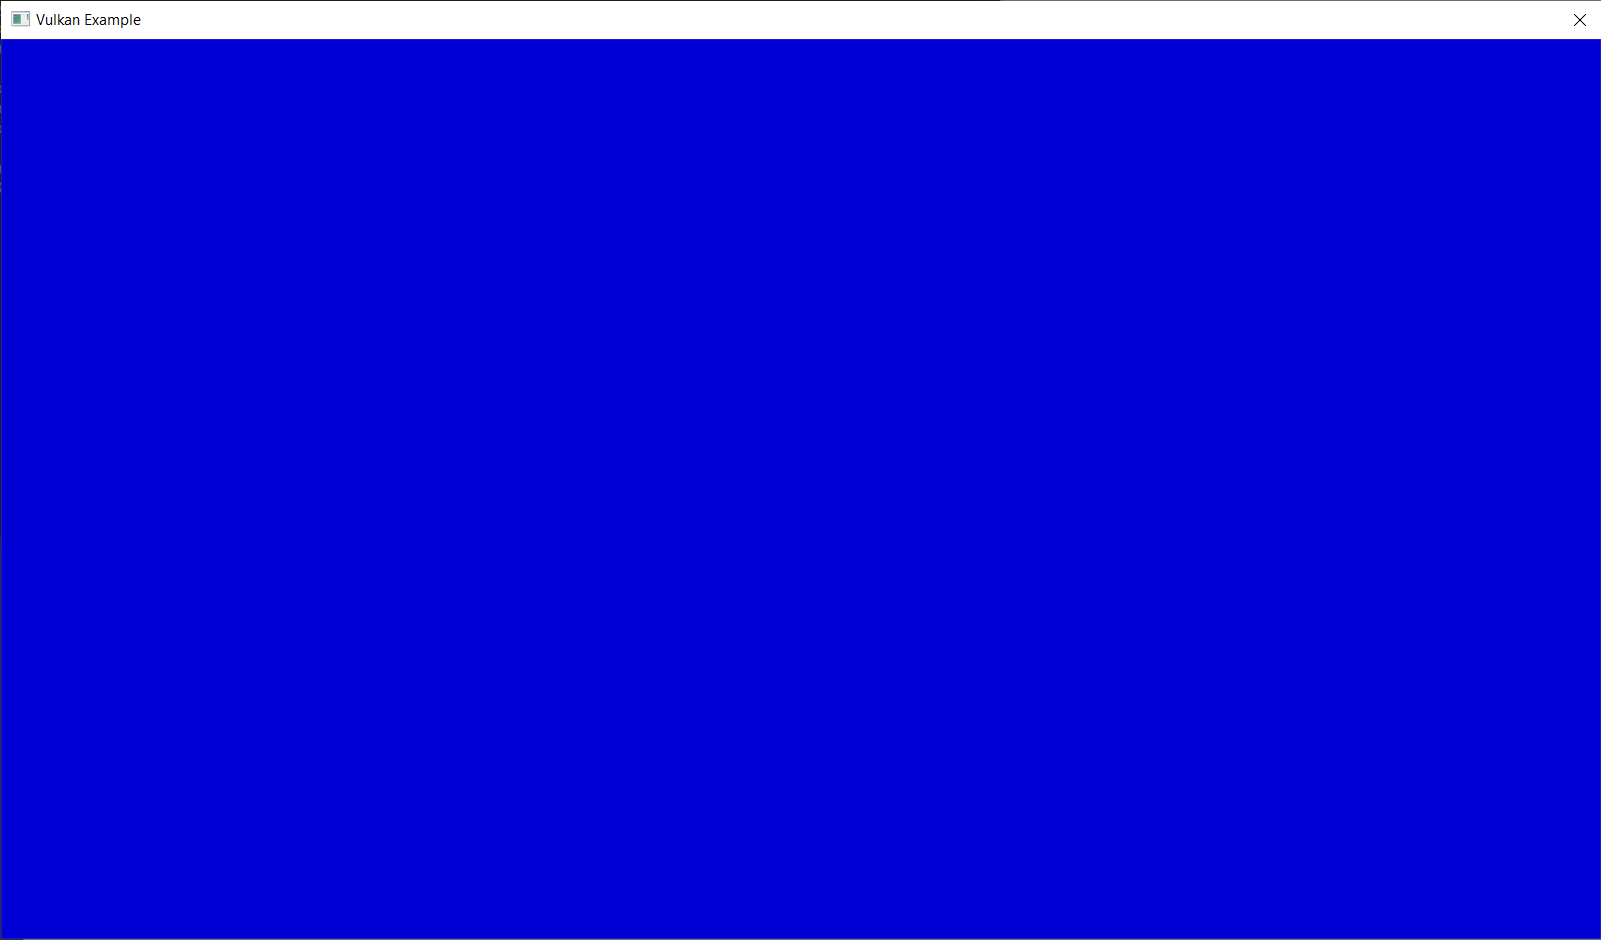
\includegraphics[scale=0.25]{images/SlidesClearWindow/ClearWindow.png}
\end{figure}

\end{frame}

% \begin{frame}
\frametitle{Setup}

\begin{itemize}
\item Creiamo due semafori: \texttt{imageAvailableSemaphore} e \texttt{renderFinishedSemaphore}
\item Li useremo per sincronizzare il rendering e la presentazione
\item Creiamo un command buffer su cui possiamo registrare dei comandi grafici
\item Creiamo una fence che useremo assieme al command buffer durante il main loop
\end{itemize}

\end{frame}

% \begin{frame}
\frametitle{Render Pass}
\begin{columns}

\column{.4\textwidth}

\begin{itemize}
\item Durante la fase di setup creiamo un render pass
\item Un render pass ci permette di descrivere le immagini (attachment) che vengono utilizzate durante il rendering
\item Un render pass suddivide le operazioni di rendering che utilizzano le stesse immagini in uno o più subpass
\end{itemize}

\column{.4\textwidth}

\begin{figure}[ht]
    \centering
    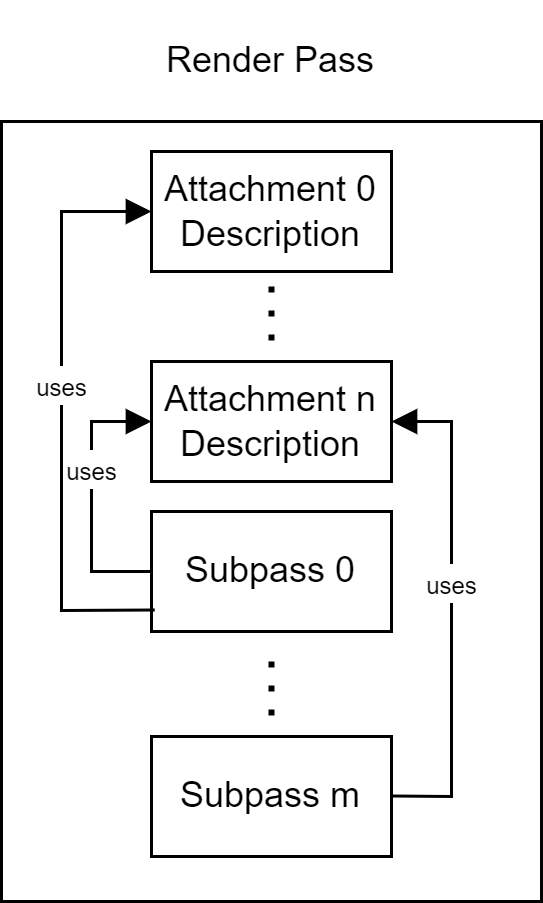
\includegraphics[scale=0.2]{images/SlidesClearWindow/RenderPass.png}
\end{figure}

\end{columns}
\end{frame}

% \begin{frame}
\frametitle{Attachmnet Description}
\begin{columns}


\column{.55\textwidth}


\begin{itemize}
\item Abbiamo un solo attachment: una delle immagini della swapchain
\item Vogliamo pulire l'attachment prima di utilizzarlo per la prima volta
\item Volgiamo mantenere il contenuto dell'attachment quando il render pass termina
\item Non ci importa del layout dell'attachment prima di iniziare il render pass
\item Quando il render pass termina, volgiamo passare a un layout che renda ottimale la presentazione dell'attachment
\end{itemize}


\column{.25\textwidth}

\begin{figure}[ht]
    \centering
    
\includegraphics[scale=0.3]{images/SlidesClearWindow/AttachmentDescription.png}
\end{figure}

\end{columns}
\end{frame}

% \begin{frame}
\frametitle{Subpass}
\begin{columns}

\column{.55\textwidth}

\begin{itemize}
\item Abbiamo un solo subpass che usa il nostro attachment
\item Durante questo subpass usiamo l'attachment come color target
\item Per questo motivo, durante questo subpass, il nostro attachment deve avere un layout adeguato
\end{itemize}

\column{.25\textwidth}

\begin{figure}[ht]
    \centering
    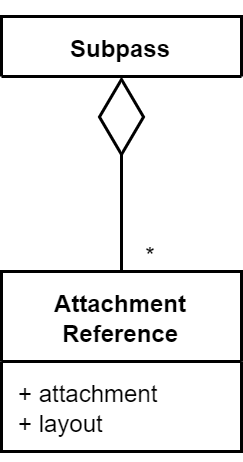
\includegraphics[scale=0.3]{images/SlidesClearWindow/Subpass.png}
\end{figure}

\end{columns}
\end{frame}

% \begin{frame}
\frametitle{Main Loop (1)}

\begin{itemize}
\item Otteniamo un'immagine dalla swapchain
\item Non è garantito che questa immagine possa essere immediatamente utilizzata
\item \texttt{imageAvailableSemaphore} viene segnalato quando l'immagine è disponibile
\item Aspettiamo che la GPU termini l'esecuzione dei comandi precedenti
\item Facciamo questo, aspettando sulla fence che abbiamo creato
\item Creiamo un framebuffer per il nostro render pass, che contiene l'immagine della swapchain che abbiamo ottenuto
\item Registriamo due comandi sul command buffer: uno per iniziare un'istanza del nostro render pass, e uno per terminarla
\item Iniziando il render pass, specifichiamo il colore da scrivere nel color target
\end{itemize}

\end{frame}

% \begin{frame}
\frametitle{Main Loop (2)}

\begin{itemize}
\item Inviamo il command buffer alla GPU
\item La GPU aspetta su \texttt{imageAvailableSemaphore} prima di iniziare l'esecuzione dei comandi
\item La GPU segnala \texttt{renderFinishedSemaphore} quando l'esecuzione dei comandi è terminata
\item Inviamo un comando di presentazione alla GPU (non ci serve un command buffer)
\item Specifichiamo l'immagine su cui abbiamo renderizzato il colore
\item La GPU aspetta su \texttt{renderFinishedSemaphore} prima di iniziare la presentazione
\end{itemize}

\end{frame}

%
% \begin{frame}
\frametitle{Demo}

\begin{figure}[ht]
    \centering
    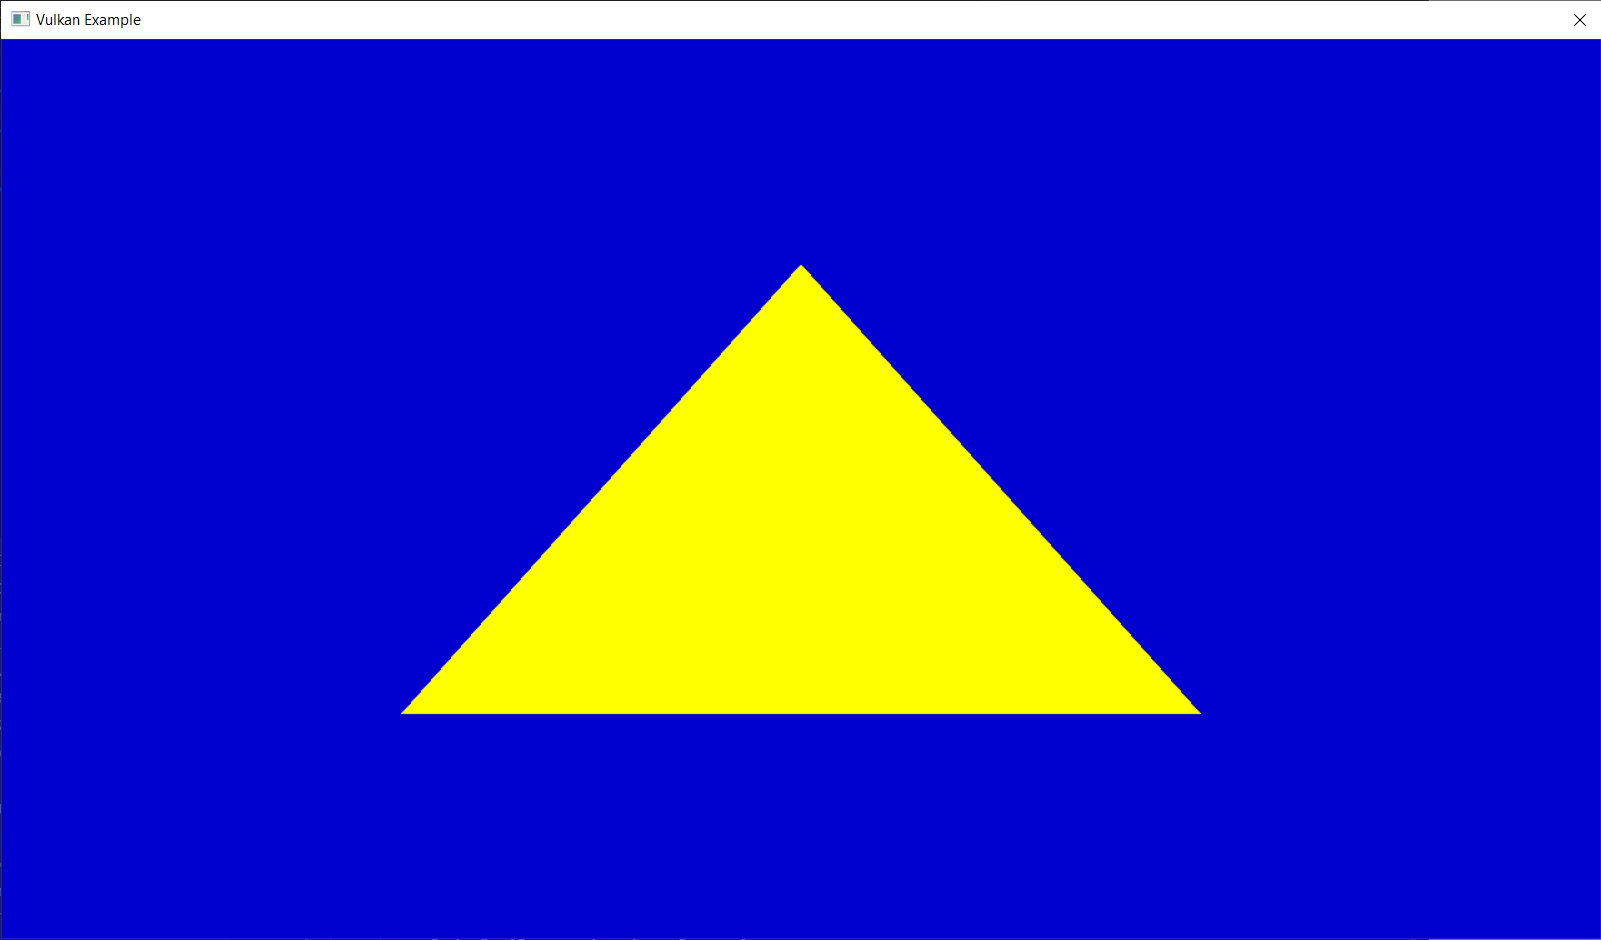
\includegraphics[scale=0.25]{images/SlidesTriangle/Triangle.png}
\end{figure}

\end{frame}

% \begin{frame}
\frametitle{Vertex Shader}

\lstinputlisting[language=C++]{src/SlidesTriangle/shader.vert}

\end{frame}

% \begin{frame}
\frametitle{Fragment Shader}

\lstinputlisting[language=C++]{src/SlidesTriangle/shader.frag}

\end{frame}

% \begin{frame}
\frametitle{Pipeline State Object}

\begin{itemize}
\item Descrive l'intero stato della pipeline grafica
\item Specifichiamo gli shader che utilizziamo per il rendering (shader stages)
\item La lista dei vertici deve essere interpretata come una lista di triangoli (input assembly)
\item Vogliamo renderizzare l'intera immagine e che non vogliamo ignorare nessun frammento generato (viewport)
\item Vogliamo generare frammenti per l'intero triangolo, non solo per i bordi (rasterization)
\item Scriviamo sull'immagine il colore di ogni frammento così com'è, senza alcuna modifica (color blend)
\end{itemize}

\end{frame}

% \begin{frame}
\frametitle{Comandi}

\begin{itemize}
\item Dobbiamo scrivere nuovi comandi nel command buffer
\item Scriviamo un comando che dice alla GPU di utilizzare il pipeline state object che abbiamo creato per configurare la pipeline grafica
\item Scriviamo un comando che dice alla GPU di attivare la pipeline grafica per renderizzare tre vertici
\end{itemize}

\end{frame}

%
% \begin{frame}
\frametitle{Demo}

\begin{figure}[ht]
    \centering
    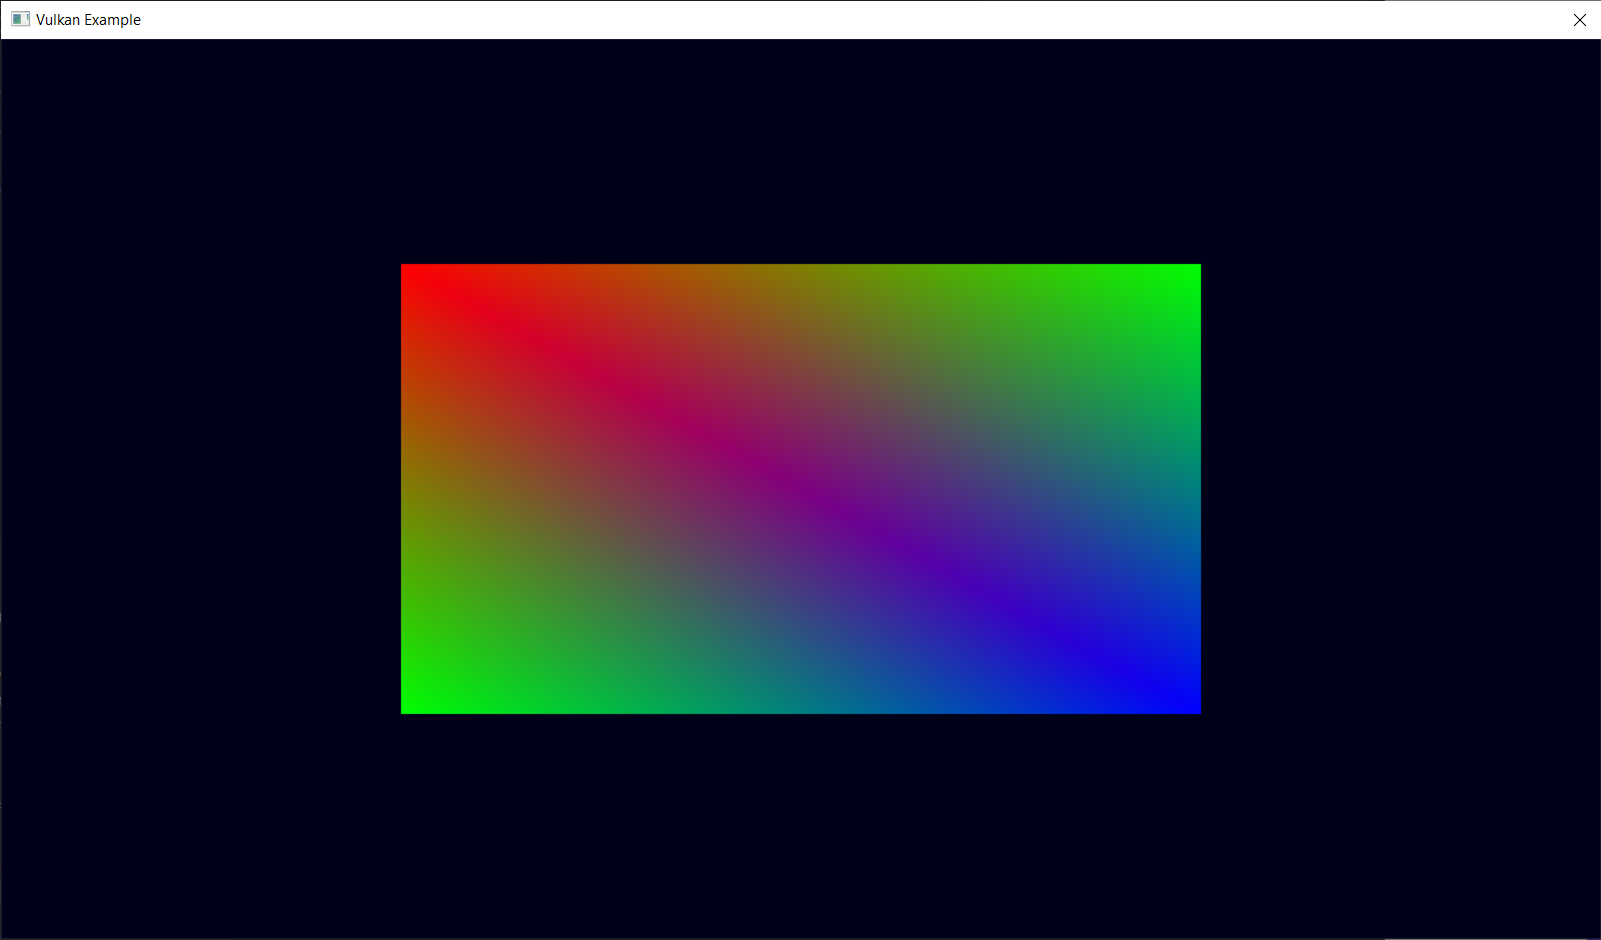
\includegraphics[scale=0.25]{images/SlidesVertices/RenderQuad.png}
\end{figure}

\end{frame}

% \begin{frame}
\frametitle{Inviare Vertici Alla GPU}

\begin{itemize}
\item Copiamo i vertici dalla RAM alla memoria della GPU
\item Usiamo due buffer allocati sulla memoria della GPU: staging buffer e vertex buffer
\item Lo staging buffer è allocato su una parte della memoria della GPU che è visibile anche dalla CPU (memoria più lenta)
\item Il vertex buffer è allocato su una parte della memoria della GPU che non è visibile dalla CPU (memoria più veloce)
\item Carichiamo i dati nello staging buffer
\item Inviamo un comando alla GPU per copiare il contenuto dello staging buffer nel vertex buffer
\end{itemize}

\end{frame}

% \begin{frame}
\frametitle{Vertex Input}

\begin{itemize}
\item Quando creiamo un pipeline state object, specifichiamo il formato dei nostri vertici
\item In questo modo, la pipeline sa come interpretare i dati che abbiamo caricato
\end{itemize}

\begin{figure}[ht]
    \centering
    
\includegraphics[scale=0.35]{images/SlidesVertices/VertexInputState.png}
\end{figure}

\end{frame}

% \begin{frame}
\frametitle{Comandi}

\begin{itemize}
\item Scriviamo un comando che dice alla GPU di utilizzare il vertex buffer creato come input per la pipeline grafica
\end{itemize}

\end{frame}

%
% \begin{frame}
\frametitle{Demo}

\begin{figure}[ht]
    \centering
    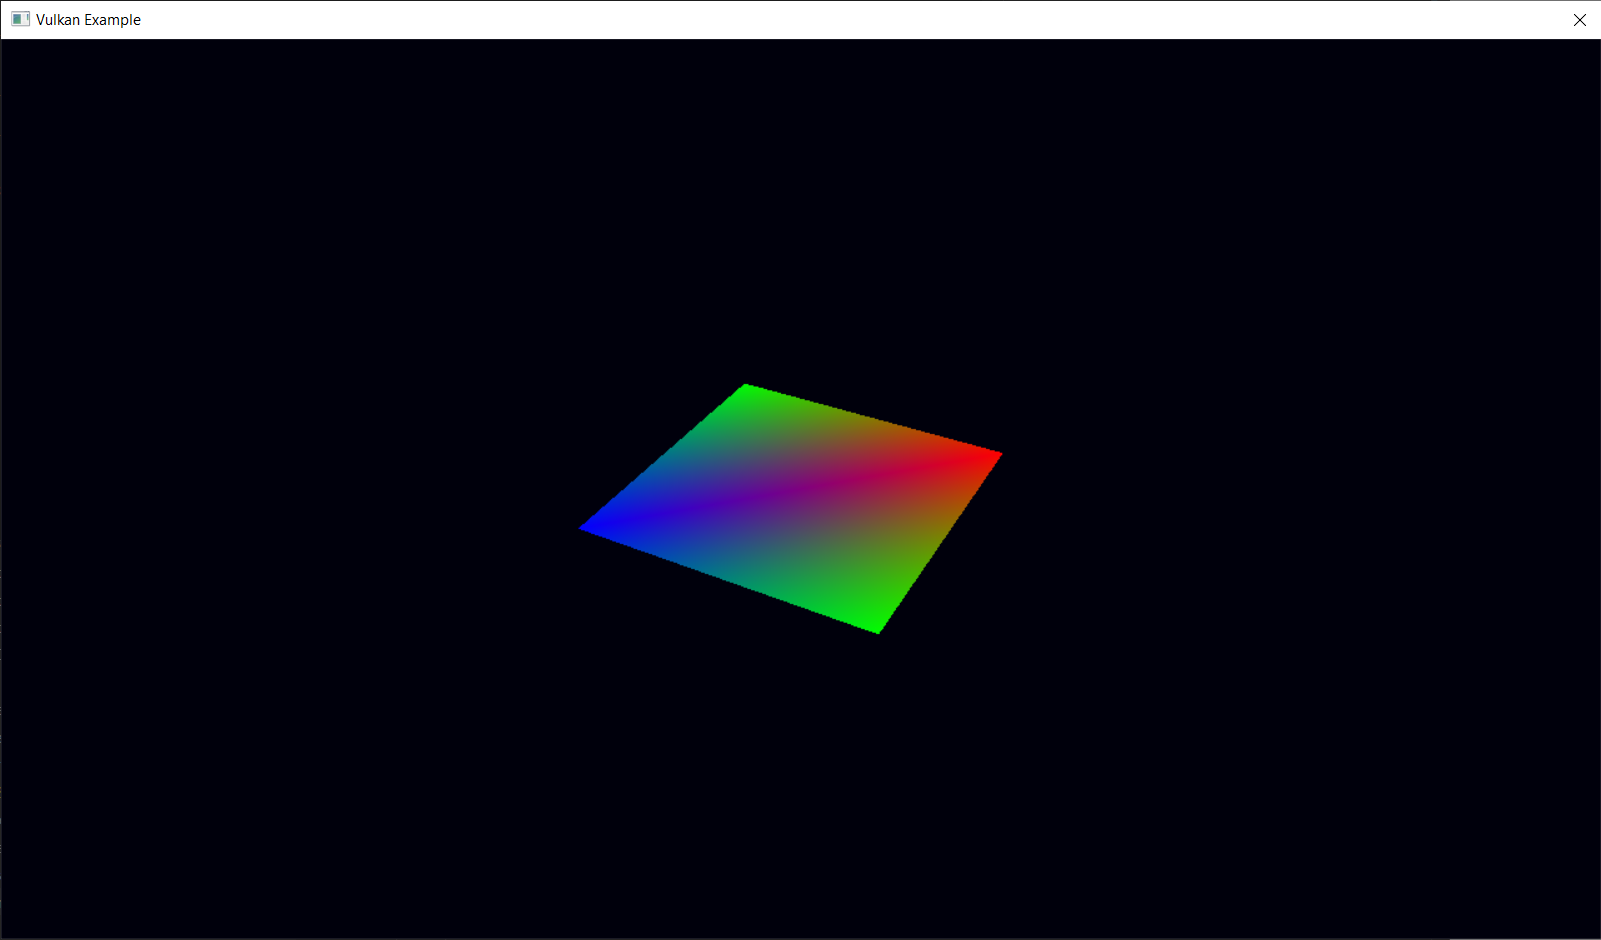
\includegraphics[scale=0.25]{images/SlidesUniforms/RenderQuad.png}
\end{figure}

\end{frame}


\begin{frame}
\frametitle{Vulkan}

\begin{itemize}
\item API grafica sotto forma di specifica
\item Non ne esiste un'unica implementazione
\item Implementata attraverso il driver della propria scheda grafica
\item Sviluppata usando come modello l'architettura delle GPU odierne
\item API di basso livello
\item Richiede un certo know how da parte del programmatore
\item Se il programmatore la utilizza in modo coscienzioso, può risultare in performance migliori rispetto alle API di vecchia generazione
\item Multithreaded first
\end{itemize}

\end{frame}

\begin{frame}
\frametitle{Inizializzare Vulkan}

\begin{itemize}
\item Creiamo una Vulkan instance
\item Creiamo una finestra (OS)
\item Creiamo una presentation surface
\item Selezioniamo una GPU (device fisico)
\item Creiamo un device logico per interfacciarsi con la GPU
\item Creiamo una swapchain per gestire la presentazione d'immagini sulla presentation surface
\end{itemize}

\end{frame}

\begin{frame}
\frametitle{Renderizzare Un Colore: Demo}
\begin{figure}[ht]
    \centering
    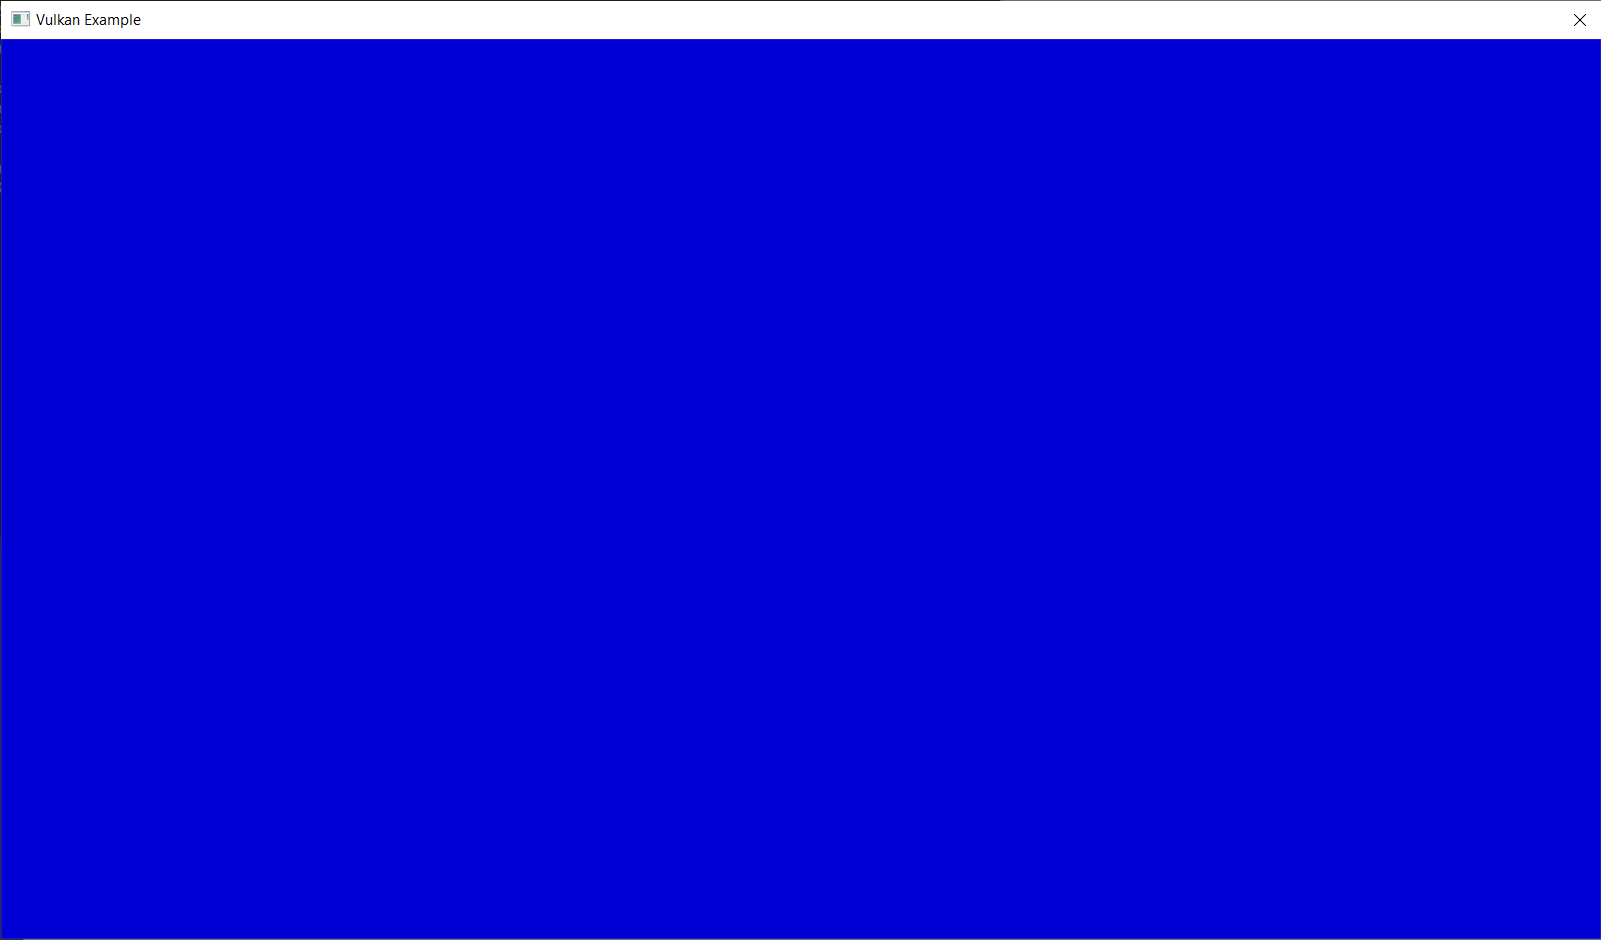
\includegraphics[scale=0.25]{images/SlidesClearWindow/ClearWindow.png}
\end{figure}
\end{frame}

\begin{frame}
\frametitle{Renderizzare Un Colore}

\begin{itemize}
\item Creiamo un render pass
\item Un render pass descrive gli attachment che vengono utilizzati durante il rendering
\item Un render pass raggruppa i comandi grafici in uno o più subpass in base a come e quali attachment utilizzano
\item Creiamo un framebuffer
\item Un reamebuffer è l'insieme di attachment utilizzati da un'istanza di un render pass
\item Creiamo un command buffer
\item Scriviamo comandi sul command buffer
\item Inviamo il command buffer alla GPU
\item Presentiamo un'immagine della swapchain sulla presentation surface
\end{itemize}
\end{frame}

\begin{frame}
\frametitle{Renderizzare Un Triangolo: Demo}
\begin{figure}[ht]
    \centering
    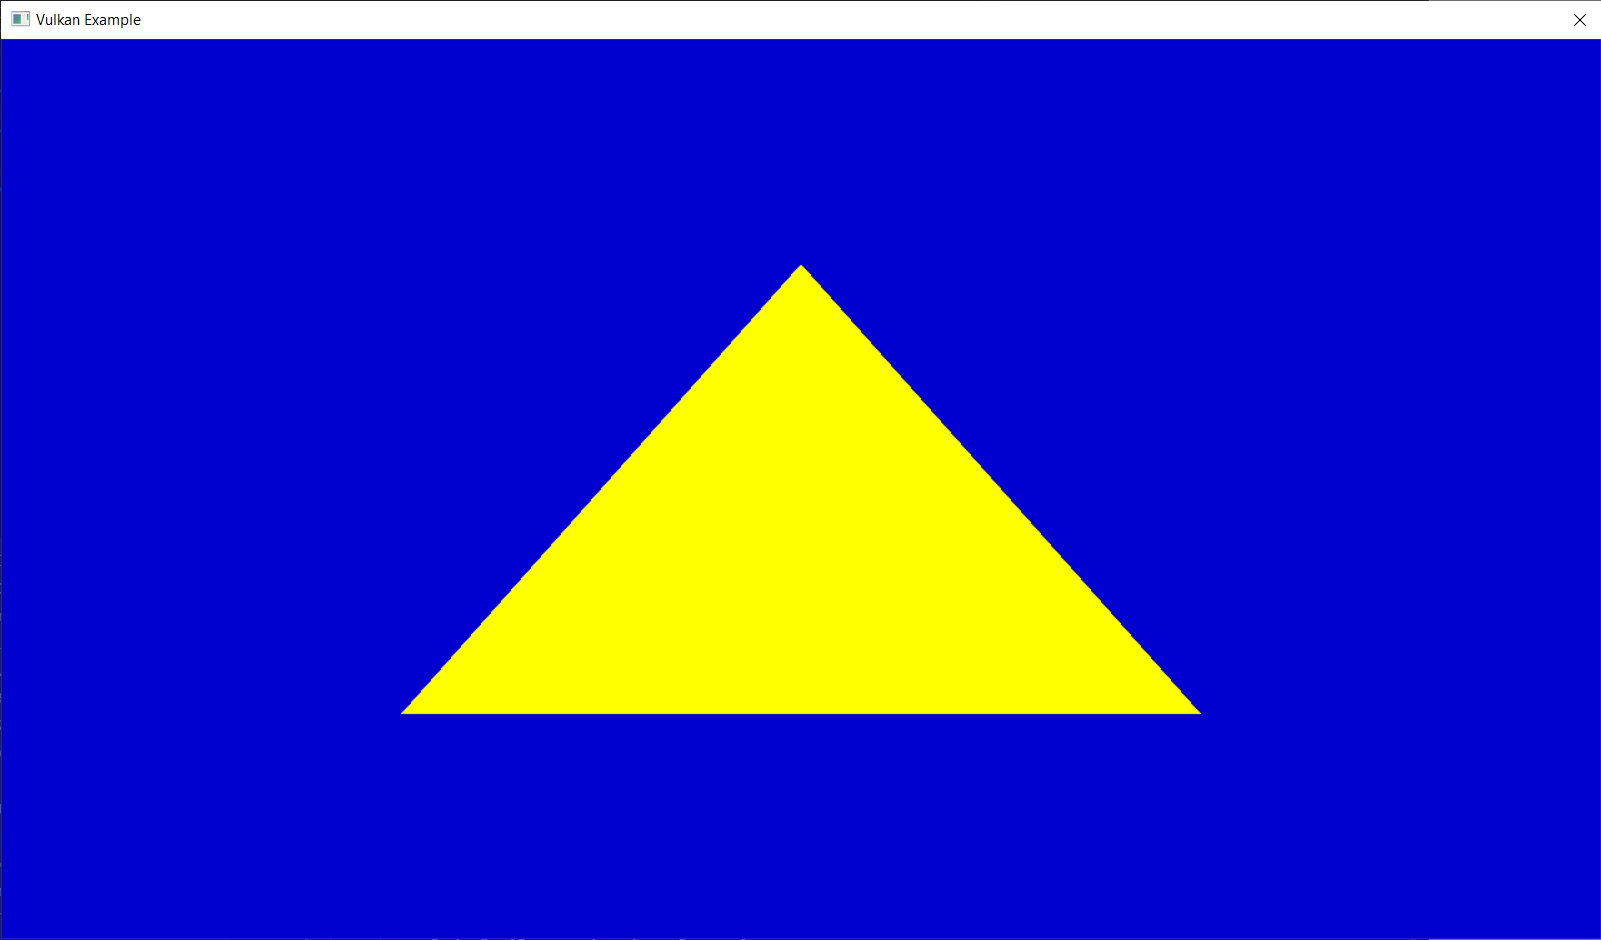
\includegraphics[scale=0.25]{images/SlidesTriangle/Triangle.png}
\end{figure}
\end{frame}

\begin{frame}
\frametitle{Renderizzare Un Triangolo}
\begin{itemize}
\item Creiamo un pipeline state object
\item Un pipeline state object descrive l'intero stato della pipeline grafica
\item Shader: programmi eseguiti dalla GPU
\item In particolare vertex shader e un fragment shader
\item La pipeline grafica riceve come input una sequenza di vertici
\item La pipeline grafica esegue il vertex shader per ogni vertice
\item Il vertex shader genera della geometria
\item La pipeline grafica esegue il fragment shader per ogni pixel coperto dalla geometria
\end{itemize}
\end{frame}

\begin{frame}
\frametitle{Vertici: Demo}
\begin{figure}[ht]
    \centering
    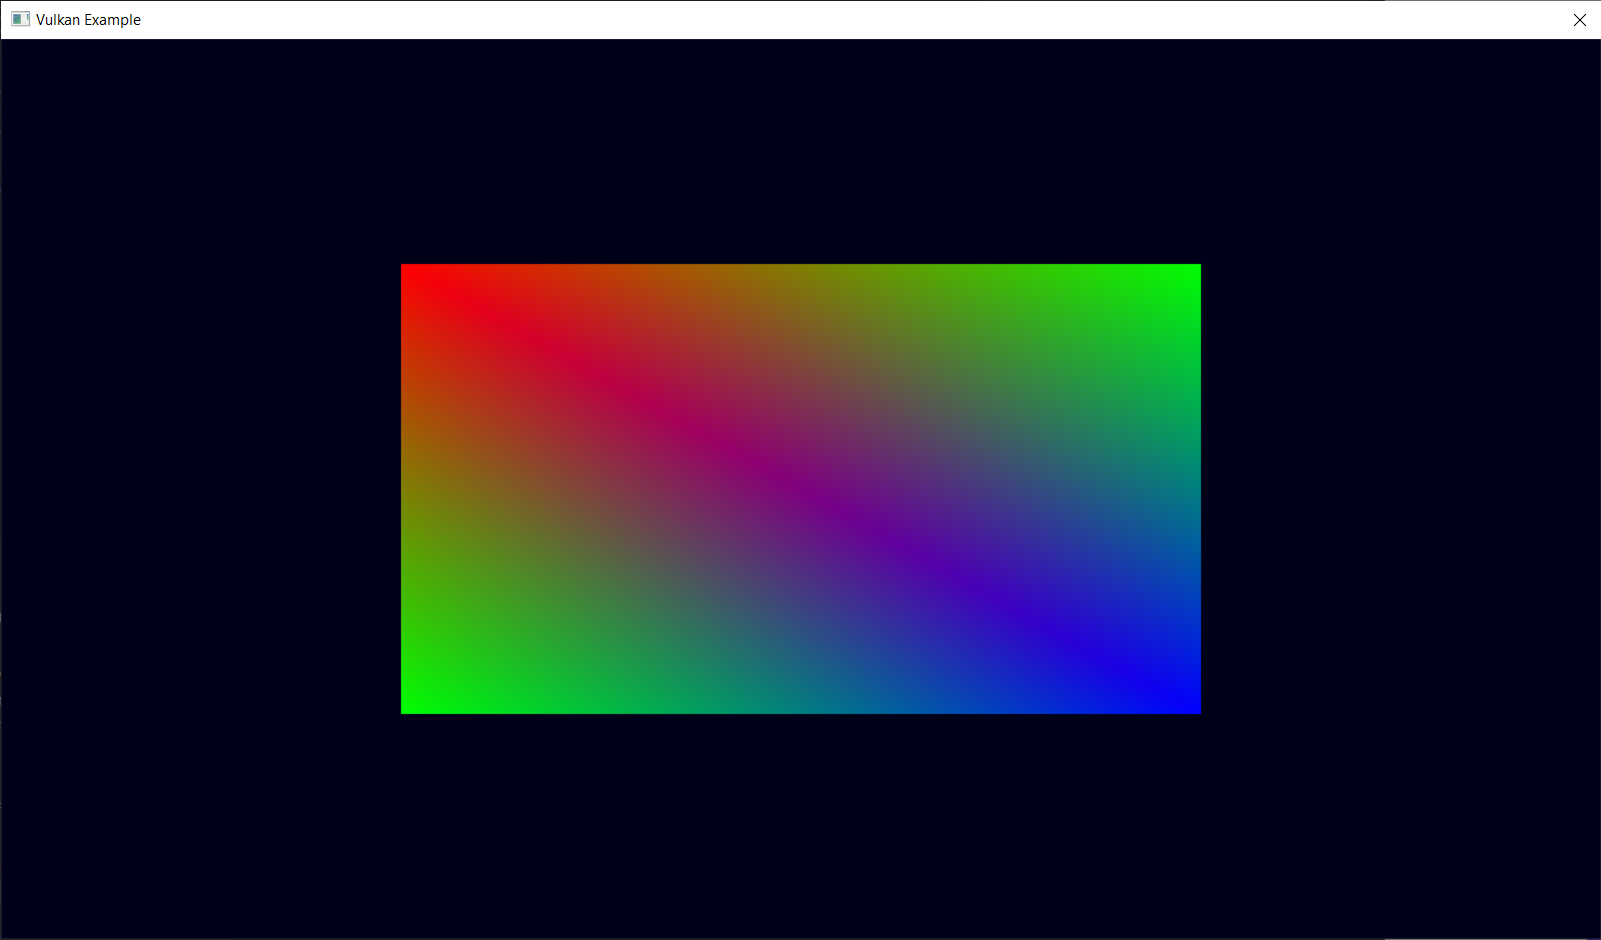
\includegraphics[scale=0.25]{images/SlidesVertices/RenderQuad.png}
\end{figure}
\end{frame}

\begin{frame}
\frametitle{Vertici}
\begin{itemize}
\item I dati dei nostri vertici sono in RAM e noi dobbiamo caricarli nella memoria della GPU
\item Usiamo due buffer
\item Uno staging buffer, allocato su memoria della GPU host visible
\item Scriviamo i dati dei nostri vertici su questo buffer
\item Un vertex buffer, allocato su memoria della GPU device local
\item Inviamo un comando che dice alla GPU di trasferire il contenuto dello staging buffer nel vertex buffer
\item Modifichiamo la creazione del nostro pipeline state object per specificare come interpretare i dati nel vertex buffer
\item Prima di registrare il comando per attivare la pipeline, registriamo un comando che indica alla pipeline grafica di usare come input il nostro vertex buffer
\end{itemize}
\end{frame}

\begin{frame}
\frametitle{Uniform Buffer: Demo}
\begin{figure}[ht]
    \centering
    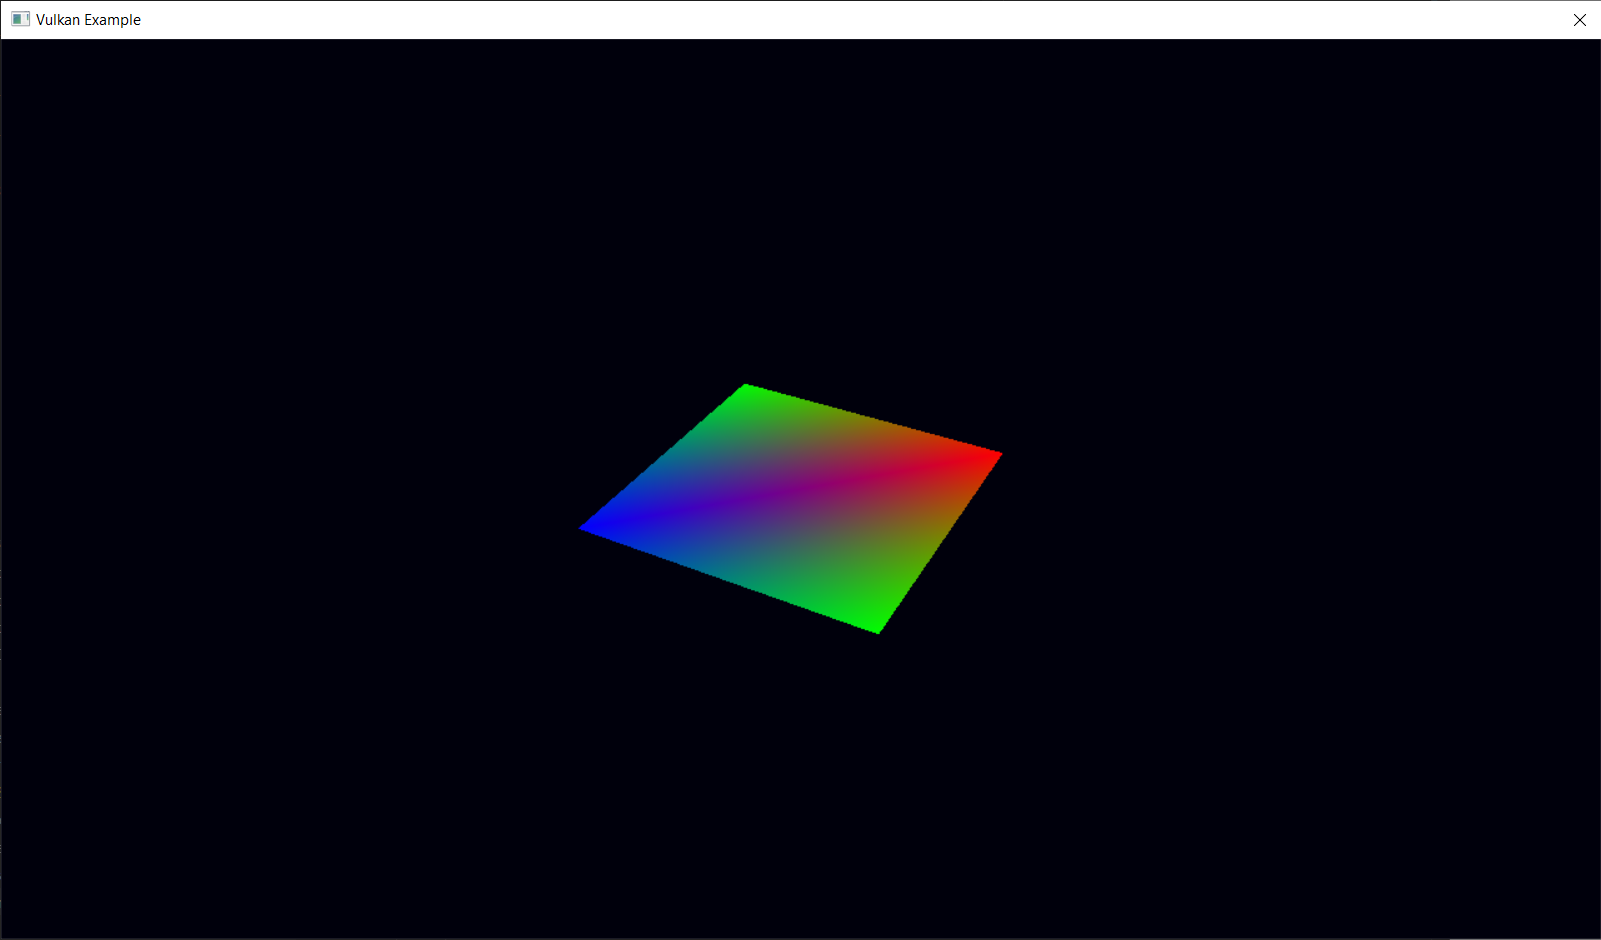
\includegraphics[scale=0.25]{images/SlidesUniforms/RenderQuad.png}
\end{figure}
\end{frame}

\begin{frame}
\frametitle{Uniform Buffer}
\begin{itemize}
\item Una variabile globale di uno shader è detta uniform
\item Passiamo le variabili globali agli shader usando uno uniform buffer
\item Siccome tali variabili cambiano frequentemente, allochiamo uno uniform buffer su memoria della GPU host visible
\item Creiamo un pipeline layout object
\item Un pipeline layout object descrive quali descriptor sono accessibili in quali shader
\item Creiamo un descriptor set layout
\item Un descriptor set layout descrive il contenuto di un descriptor set
\item Creiamo un descriptor set basandoci sul descriptor set layout
\item Una volta allocato, un descriptor set va popolato con i descriptor appropriati
\end{itemize}
\end{frame}

\begin{frame}
\frametitle{Depth Buffer: Demo}

\begin{columns}

\column{.5\textwidth}

\begin{figure}[ht]
    \centering
    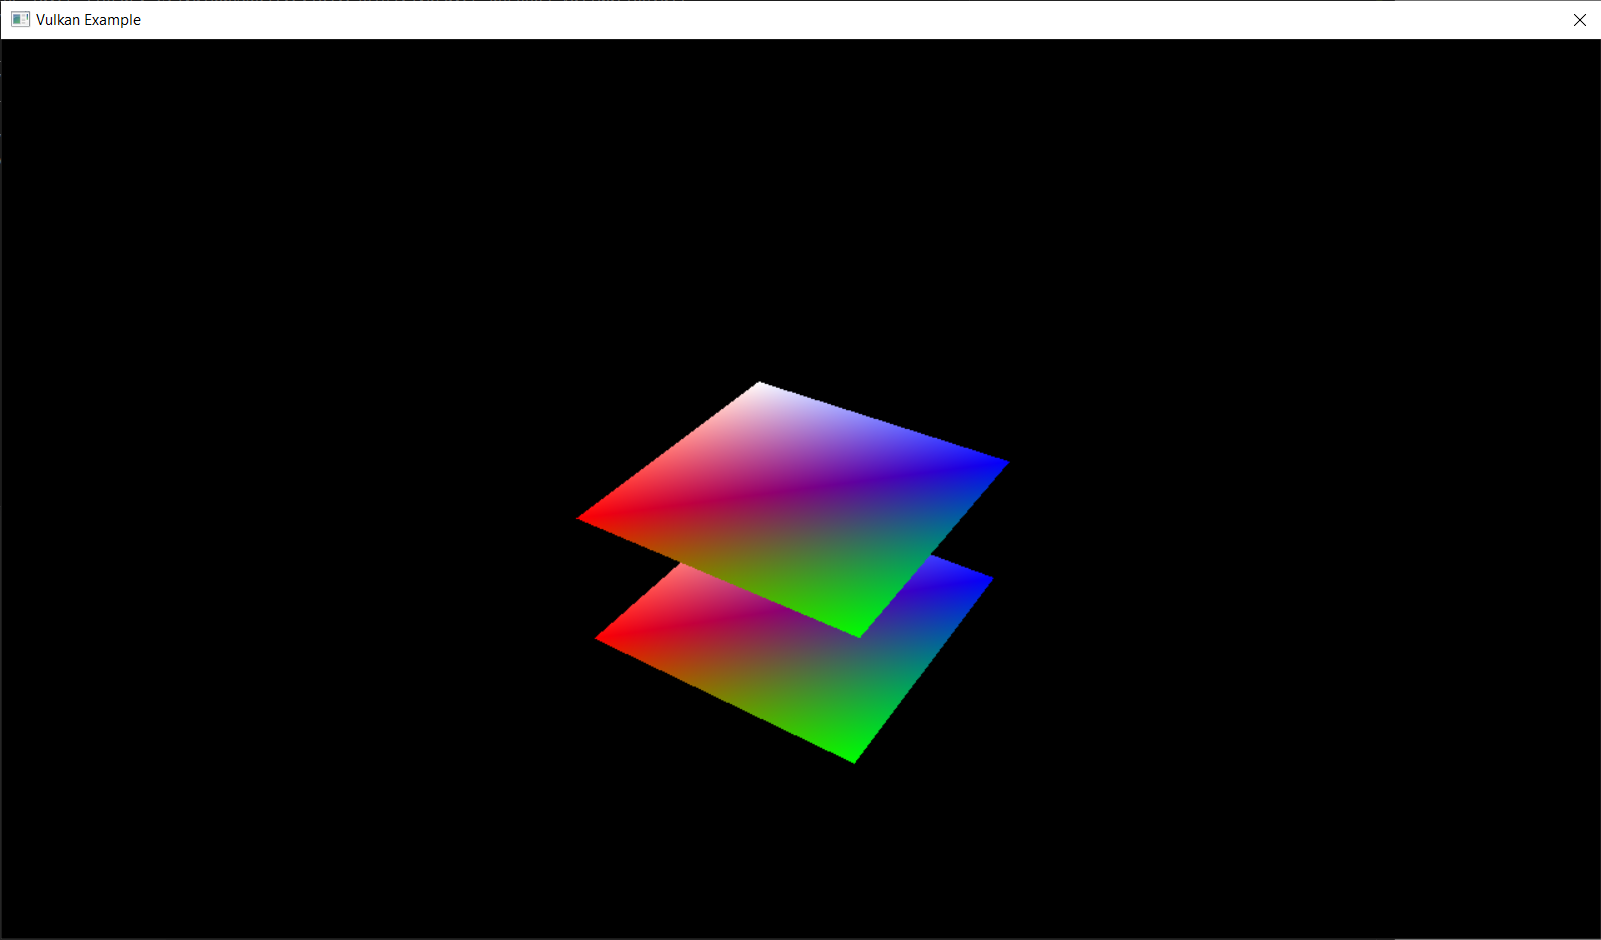
\includegraphics[scale=0.14]{images/SlidesDepthTesting/DepthTesting.png}
\end{figure}

\column{.5\textwidth}

\begin{figure}[ht]
    \centering
    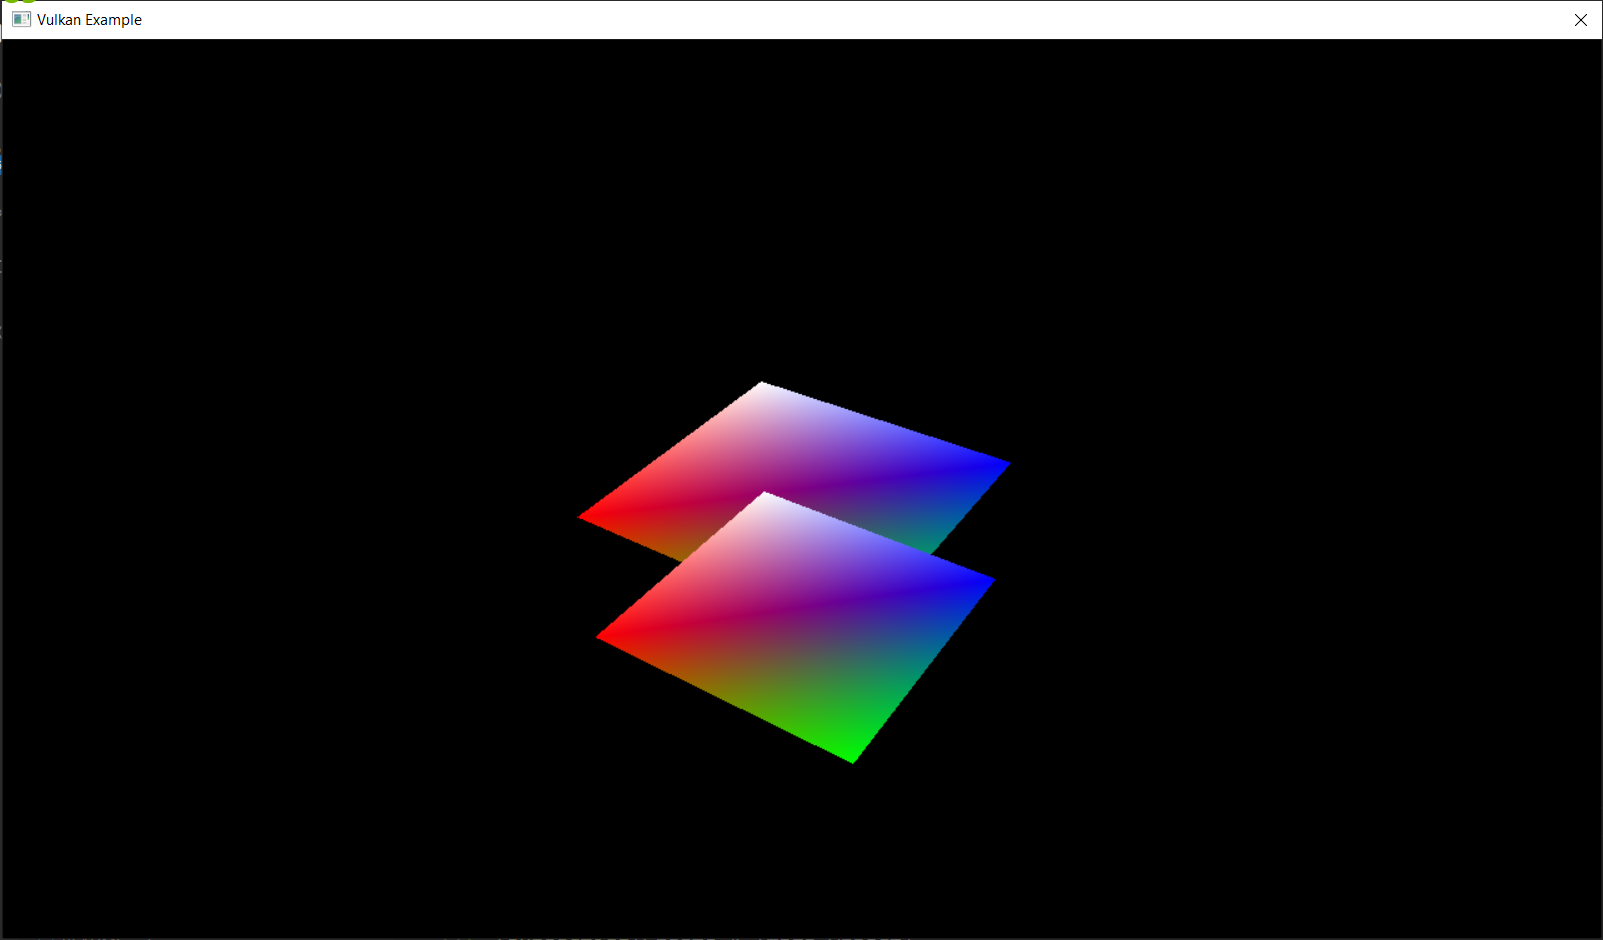
\includegraphics[scale=0.14]{images/SlidesDepthTesting/NoDepthTesting.png}
\end{figure}

\end{columns}

\end{frame}

\begin{frame}
\frametitle{Depth Buffer}
\begin{itemize}
\item Come renderizzare oggetti in modo tale che quelli più vicini possano nascondere quelli più lontani?
\item Possiamo ordinare gli oggetti in base alla loro lontananza dalla camera
\item E se due oggetti si sovrappongono?
\item Se gli oggetti da renderizzare sono opachi, usiamo un depth buffer
\item Un depth buffer è un'immagine che codifica informazioni riguardanti la profondità dei frammenti
\item Quando un frammento viene generato, compariamo la sua profondità con quella salvata nel corrispettivo texel del depth buffer
\item Se è più grande, il frammento non viene ignorato
\item Se è più piccola, il frammento viene utilizzato e la sua profondità viene salvata nel depth buffer
\item Creiamo un'immagine da usare come depth stencil attachment
\item Abilitiamo il depth testing quando creiamo il pipeline state object
\end{itemize}
\end{frame}

\begin{frame}
\frametitle{Scene}
\begin{columns}


\column{.6\textwidth}


\begin{itemize}
\item
\end{itemize}


\column{.2\textwidth}


\end{columns}
\end{frame}

\begin{frame}
\frametitle{Blinn-Phong: Demo}
\begin{figure}[ht]
    \centering
    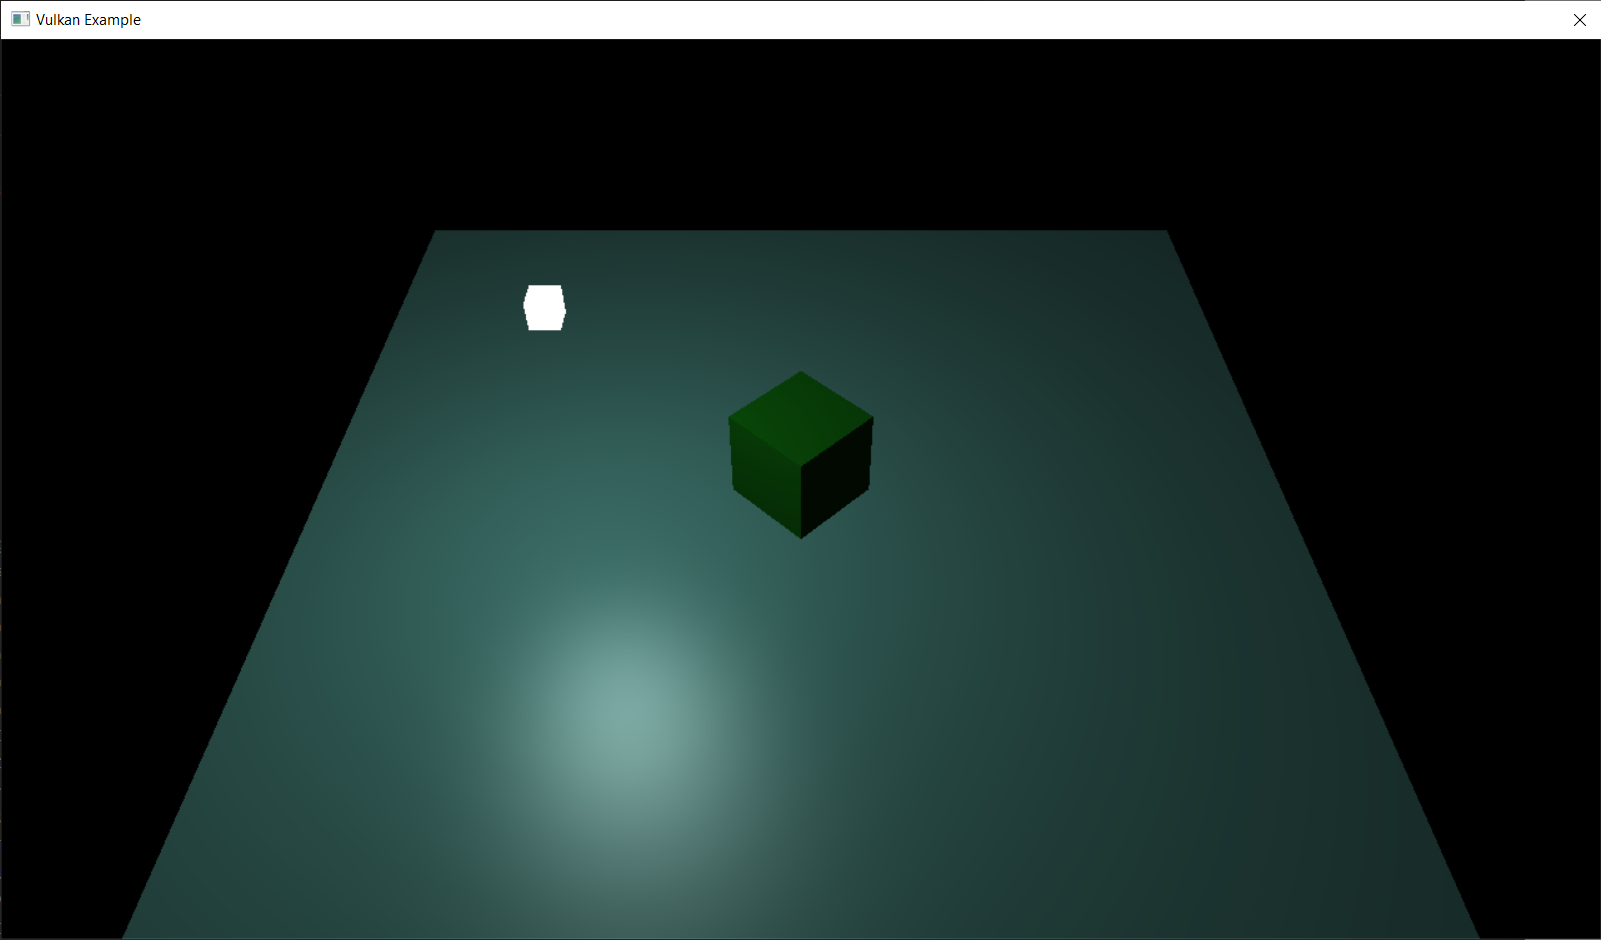
\includegraphics[scale=0.25]{images/SlidesBlinnPhong/SceneMaterialsLight.png}
\end{figure}
\end{frame}

\begin{frame}
\frametitle{Blinn-Phong}
\begin{itemize}
\item L'illuminazione viene divisa in tre componenti: ambient, diffuse e specular
\item La componente ambientale modella il fatto che una scena non è mai totalmente buia
\item La componente diffusiva simula l'impatto che la luce ha sugli oggetti opachi
\item La componente speculare simula il punto luminoso che una luce causa su oggetti lucidi (specular highlight)
\item Ogni oggetto ha un materiale: componente ambientale, diffusiva, speculare e lucentezza
\item Una luce ha diverse intensità per la componente ambientale, diffusiva e speculare
\end{itemize}
\end{frame}

\begin{frame}
\frametitle{MSAA: Demo}
\begin{figure}[ht]
    \centering
    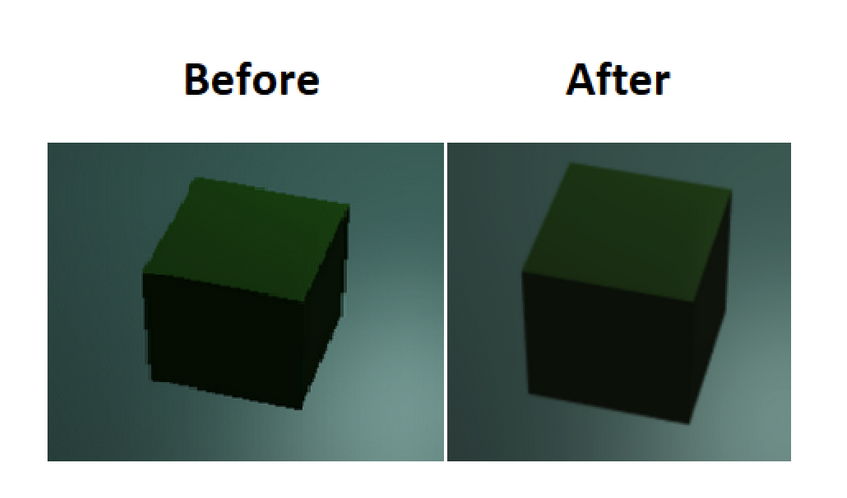
\includegraphics[scale=0.50]{images/SlidesMSAA/BeforeAfterMSAA.png}
\end{figure}
\end{frame}

\begin{frame}
\frametitle{MSAA: Un Campione Per Pixel}
\begin{figure}[ht]
    \centering
    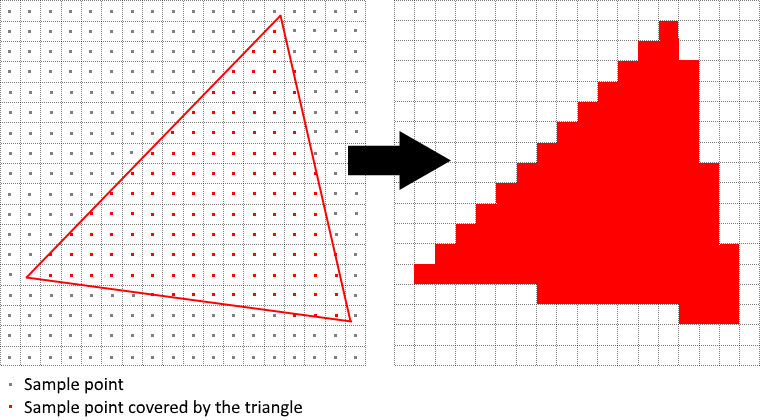
\includegraphics[scale=0.50]{images/SlidesMSAA/OneSamplePerPixel.png}
\end{figure}
\end{frame}

\begin{frame}
\frametitle{MSAA: Quattro Campioni Per Pixel}
\begin{figure}[ht]
    \centering
    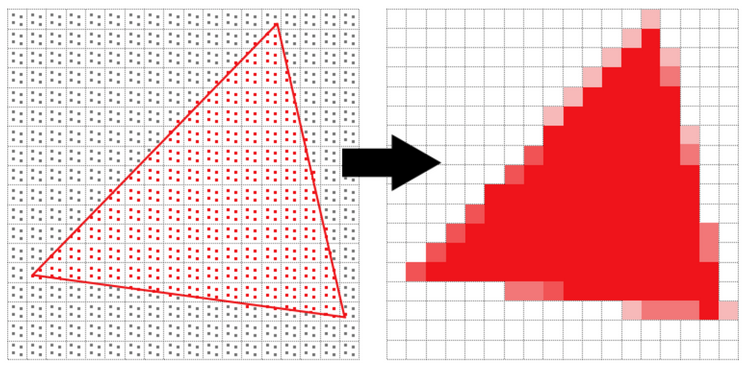
\includegraphics[scale=0.50]{images/SlidesMSAA/FourSamplesPerPixel.png}
\end{figure}
\end{frame}

\begin{frame}
\frametitle{MSAA}
\begin{itemize}
\item Le immagini che supportano il multisampling non sono presentabili
\item Tutte le immagini presentabili devono avere un solo campione per pixel
\item Creiamo una nuova immagine che abbia il numero di campioni per pixel che desideriamo
\item Useremo questa immagine come nuovo color attachment nel render pass
\item Usiamo l'immagine della swapchain come color resolve attachment
\item Non dobbiamo dimenticarci di abilitare l'uso del multisampling quando creiamo un pipeline state object
\end{itemize}
\end{frame}


\end{document}
